\documentclass[12pt,a4paper]{article}
\usepackage{lmodern}
\usepackage[utf8]{inputenc}
\usepackage[T1]{fontenc}
\usepackage{geometry}
\usepackage{setspace}
\usepackage{graphicx}
\geometry{a4paper, total={170mm,257mm}, left=20mm, top=20mm}

\title{\Huge BaDMat 1.0 \\ \LARGE Mode d'emploi} % Ça fait un peu BatMan, on garde vraiment ce nom-là ?
\author{Myrtille Grulois \thanks{Université populaire et citoyenne de Roubaix}}
\date{Été 2020}

\renewcommand*\contentsname{Sommaire}

\begin{document}

\begin{titlepage}
\maketitle
\end{titlepage}

\tableofcontents
\clearpage

\addcontentsline{toc}{section}{Introduction}
\section*{Introduction}

Ce manuel d'utilisation concerne la première version du logiciel BaDMat de l'UPC de Roubaix.
Les explications concernent à la fois la structure de la base de donées et les différentes fonctions disponibles.
Pour toute action d'ordre général, se reporter au préambule, qui contient des instructions valables pour la plupart des fonctions (sauf mention contraire).

\bigskip
\section{Préambule : ce qu'il est utile de savoir (faire)}

\subsection{Ouverture du terminal}

    Bon je vais pas trop détailler, comme on n'a pas encore décidé de l'OS à utiliser\dots
    À mettre à jour.

\subsection{Lancement d'un script}
    Tout d'abord, précisons que dans notre cas, un script correspond à une fonctionnalité.
    Chaque fonction décrite ci-dessous est donc lancée à partir d'un fichier différent.
    Pour lancer un script (à compléter, dépend 1. de l'OS 2. de comment fonctionne Python sur l'OS)

\subsection{Utilisateurs et connexion à la base de données}
    À compléter une fois qu'on aura discuté des mots de passe

\subsection{Interactions avec le programme}
    Pour la plupart des instructions, le programme nécessite que vous rentriez une lettre en majuscule.
    Tapez la lettre correspondant à votre choix parmi les propositions de la question,
    puis validez en tapant "Entrée".

\subsection{Définition des termes utilisés}
    Tout au long de la suite, ligne désignera une entrée dans la base de données.
    Colonne désignera un des possibles critères de cette ligne.
    
    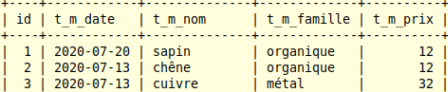
\includegraphics{exemple_lignes_colonnes.png}

    Dans l'exemple ci-dessus, la ligne d'ID 1 décrivant le sapin est nommée\dots ligne.
    On nommera colonne, par exemple, le critère ID. Pour aller plus loin, la colonne ID
    est de type numérique, tandis que la colonne t\_m\_famille est de type textuel.



\bigskip
\section{Fonctions}

Cette section regroupe les différentes fonctions implémentées, ainsi que la façon de les exécuter, et les différentes options possibles.


\subsection{Recherche}

    La fonction principale de cette base de données est la fonction de recherche.
    Pour l'exécuter, lancer le script \emph{search.py}, puis se connecter à la base de données.
    Il existe deux types de recherche : la recherche simple et la recheche avancée.

    \subsubsection{Recherche simple}
        La recherche simple est à privilégier si vous ne souhaitez inclure qu'une seule colonne dans votre recherche.
        Vous aurez toujours la possibilité de choisir quelle(s) colonne(s) vous souhaitez afficher dans les résultats.


        \medskip
        \textbf{Recherche textuelle}

        Si la colonne que vous sélectionnez est de type textuel, alors vous pourrez entrer un mot ou une expression.
        
        \medskip
        \textbf{Recherche numérique}
        
        Si la colonne que vous sélectionnez est de type numérique, vous pourrez effectuer une recherche autour d'une valeur donnée,
        ou bien une recherche sur un intervalle. Si vous choisissez la recherche numérique simple, vous aurez toutefois
        la possibilité d'entrer une tolérance. La recherche s'effectuera alors sur l'intervalle de longueur de deux fois votre tolérance
        qui entoure votre valeur.

        \medskip
        \textbf{Recherche par date}
        
        Vous pouvez également effectuer une recherche sur la date.

    \subsubsection{Recherche avancée}
        La recherche avancée vous prendra plus de temps. Elle permet à la fois d'effectuer une recherche sur plusieurs colonnes,
        mais également de rechercher plusieurs critères dans la même colonne (pour les colonnes de texte).

        \medskip
        \textbf{Recherche textuelle}

        Si la colonne que vous sélectionnez est de type textuel, alors vous pourrez entrer un mot ou une expression, qui sera recherché
        dans cette colonne. Toutefois, vous aurez ensuite la possibilité d'ajouter des mots supplémentaires, que vous pourrez moduler :
        c'est-à-dire imposer que le mot saisi ne se trouve pas dans les résultats de votre recherche, ou bien cherche le premier terme
        ou bien le deuxième, etc.
        
        \medskip
        \textbf{Recherche numérique}
        
        La recherche numérique avancée est identique à celle de la recherche simplifiée.
        Si la colonne que vous sélectionnez est de type numérique, vous pourrez effectuer une recherche autour d'une valeur donnée,
        ou bien une recherche sur un intervalle. Si vous choisissez la recherche numérique simple, vous aurez toutefois
        la possibilité d'entrer une tolérance. La recherche s'effectuera alors sur l'intervalle de longueur de deux fois votre tolérance
        qui entoure votre valeur.

        \medskip
        \textbf{Recherche par date}
        
        Vous pouvez également effectuer une recherche sur la date.






\section{Base de données}

\subsection{Structure de la base de données}

\begin{verbatim}
    Test de code Blablabla
    Deuxième ligen
    Là je laisse une indentation
    for i in range(0, 3):
\end{verbatim}


\end{document}